\documentclass[titlepage=firstiscover, captions=tableheading, bibliography=totoc]{scrartcl}

\usepackage{polyglossia}
\setmainlanguage{german}

\usepackage{fontspec}
\usepackage{amsmath}
\usepackage{amssymb}
\usepackage{mathtools}
\usepackage[locale=DE, separate-uncertainty=true, per-mode=symbol-or-fraction]{siunitx}
\usepackage{microtype}
\usepackage{xfrac}
%\usepackage{subcaption}
%\usepackage{graphicx}
%\usepackage{grffile}
\usepackage{booktabs}
\usepackage{biblatex}
\addbibresource{litvz.bib}

\usepackage{lscape}

\usepackage[math-style=ISO,bold-style=ISO,sans-style=italic,nabla=upright,partial=upright,]{unicode-math}
\setmathfont{Latin Modern Math}

\begin{document}
\setlength{\parindent}{0em}

%\pagestyle{empty}
%Keine Seitenzahl

%\newcommand{\Titel}{Optisches Pumpen}
\newcommand{\DatumDu}{07. November 2018}
\newcommand{\DatumAb}{??. November 2018}
\newcommand{\Autoreins}{Katharina Brägelmann}
\newcommand{\Emaileins}{katharina.braegelmann@tu-dortmund.de}
\newcommand{\Autorzwei}{Tobias Janßen}
\newcommand{\Emailzwei}{tobias2.janssen@tu-dortmund.de}



\begin{titlepage}

\begin{center} \large

  FP
  \vspace*{2.5cm}
  %\vspace=platz bis zur nächsten Zeile

  {\huge \Titel}
  \vspace*{3cm}

  \Autoreins
  \\\Autorzwei
  \vspace*{1.5cm}

  \Emaileins, \Emailzwei


  Durchführung: \DatumDu, Abgabe: \DatumAb
  \vspace*{4.5cm}


\end{center}
\end{titlepage}

%\input{lit.bib}
\pagenumbering{arabic}

\tableofcontents
\newpage

\section{Zielsetzung}
\input{Zielsetzung.txt}


\section{Theorie}
Bei der Sonographie werden Schallwellen zwischen $\SI{20}{kHz}$ bis $\SI{1}{GHz}$ verwendet.
Dabei handelt es sich bei Schall um eine longitudinale Welle der Form:
\begin{align*}
  p(x, t)= p_{\text{0}}-v_{\text{0}}Z \cos{(\omega t -k x)}.
\end{align*}
$Z$ beschreibt dabei die akustische Impedanz $Z=c \cdot \rho$, also das Produkt aus Schallgeschwindigkeit $c$ und der Dichte $\rho$ des durchschallten Mediums.
Näheres kann in der Theorie zu Versuch US2 nachgelesen werden.\\
Bewegen sich Schallquelle und Beobachter relativ zu einander, kommt es zu einer Frequenzänderung, die als der Doppler-Effekt bekannt ist.
Die Frequenz $\nu_0$ wird zu Frequenz $\nu_{\text{kl}}$ erhöht wenn sich die Quelle auf den Beobachter zu bewegt.
Entfernt sich die Quelle vom Beobachter, wird die Frequenz $\nu_{\text{gr}}$ wahrgenommen.
\begin{align*}
  \nu_{\text{kl/gr}}=\frac{\nu_0}{1\mp\frac{v}{c}}
\end{align*}
Wird nun der Beobachter auf die Quelle zu bewegt, wird die Frequenz $\nu_0$ zu Frequenz $\nu_{\text{h}}$ verschoben.
Bei steigender Entfernung wird die Frequenz kleiner zu dem Wert $\nu_{\text{n}}$.
\begin{align*}
  \nu_{\text{h/n}}=\nu_0\cdot\left(1\pm\frac{v}{c}\right)
\end{align*}
Über die Frequenzverschiebung kann eine Aussage zur Geschwindigkeit gemacht werden.
Da die Quelle im selben Winkel zum bewegten Objekt steht wie der Empfänger, gilt für den Doppler-Effekt folgender Zusammenhang:
\begin{align}
  \Delta \nu = 2 \nu_0 \frac{v}{c}  \text{cos} \alpha
  \label{eqn:v}
\end{align}
\\ Die Schallwellen werden häufig durch den Piezo-elektrischen Effekt erzeugt.
Dabei wird ein Piezokristall durch ein wechselndes elektrisches Feld in Schwingung gebracht.
Diese Wellen können als Ultraschall für die Untersuchung genutzt werden.
Wird die Resonanzfrequenz des Kristalls erreicht, entstehen durch die Resonanzüberhöhung energiereiche Schallwellen.
Andersherum kann ein ruhender Piezokristall durch eine Schallwelle in Schwingung gebracht werden,
die dann als Spannung in das elektrische Feld eingehen.
Damit kann der Piezo-elektrische Effekt sowohl für den Ultraschallsender und den Ultraschallempfänger verwendet werden.



\section{Aufbau und Durchführung}
Auf einer zweifach eingespannten, drehbaren Achse können verschiedene Körper befestigt werden.
Die Achse ist über eine Feder mit dem Rahmen verbunden.
Zur Berechnung späterer Trägheitsmomente werden die Konstanten der Feder benötigt.
\\D wird bestimmt, indem eine Federwaage an einem bestimmten Abstand zur Achse an eine nahezu masselosen Stange ansetzt wird und diese Stange den Winkel $\phi$ ausgelenkt wird.
An der Federwaage ist die zugehörige Kraft ablesbar.
Es wird die Kraft für 10 Winkel gemessen.
\\Das Eigenträgheitsmoment $I_D$ wird bestimmt, indem eine Stange mit zwei zylinderförmigen Gewichten senkrecht zur Drillachse befestigt wird und diese in Schwingung versetzt wird.
Die Schwingungsdauer ist für 10 unterschiedliche Abstände der Massen zur Drehachse zu messen.
\\Anschließend wird das Trägheitsmoment von einem liegenden und einem stehenden Zylinder ermittelt.
Dafür wird wieder die Schwingungsdauer der Körper gemessen.
\\Eine Holzpuppe wird nach der Vermessung ihrer Proportionen und nach Messen des Gewichtes, auf die Drillachse gesteckt.
Es werden für zwei verschiedenen Körperhaltungen die Schwingungszeiten ermittelt.
Zunächst werden die Schwingungsdauern der Puppe mit angelegten Armen gemessen, dann werden die Schwingungsdauern der selben Puppe mit seitlich ausgestreckten Armen gemessen.

\newpage

\section{Auswertung}
\subsection{Einregeln der optimalen Verzögerungszeit}
Da die Leitungen von den SEV zur Koinzidenzschaltung nicht zwingend gleich schnell sind, wird die Verzögerung zwischen den beiden Seiten optimiert.
Die Verzögerungszeit kann in beiden Leitungen separat erhöht werden, indem Kabel mit definierten Verzögerungen zugeschaltet werden.
Eine Verzögerung bei der einen Kabelleitung bewirkt eine relative 'Beschleunigung' der anderen Kabelleitung.
Die Zählrate $N$ wird in Abhängigkeit verschiedener Verzögerungszeiten $T_{\text{VZ}}$ gemessen (Tabelle \ref{tab:verzögerung}, Abbildung \ref{fig:verzögerung}).
\input{tabelleverzögerung.tex}
\begin{figure}[h!]
  \centering
  \includegraphics[width=\textwidth]{figverzögerung.pdf}
  \caption{Optimierung der Verzögerungszeit: Verzögerungszeit $T_{\text{VZ}}$ gegen die Zählrate $N$}
  \label{fig:verzögerung}
\end{figure}
Es wird eine Ausgleichsrechnung der Form
\begin{equation*}
  N = -a \left( T_{\text{VZ}} +b \right)^4+c
\end{equation*}
mit Python 3.6.3 vorgenommen.
Die Parameter ergeben sich zu
\begin{align*}
  a &=& \SI{  4.8215 \pm 0.2361 e41}{\frac{1}{s^5}}\\
  b &=& \SI{  2.0854 \pm 0.2292 e-9}{s}\\
  c &=& \SI{208.0012 \pm 3.5037 e9}{\frac{1}{s}}.\\
\end{align*}
Dabei beschreibt $b$ die seitliche Verschiebung des Maximums und damit den Wert, der fortan als Verzögerung der Leitung gewählt wird.
Damit sind die Signale aus den SEV annähernd gleichzeitig an der Koinzidenzschaltung. $c$ ist die berechete maximale Zählrate.\\
Desweiteren wird die Halbwertsbreite der Zählrate bestimmt.
Die Halbwertsbreite ist im Diagramm durch eine Konstante bei $\frac{c}{2}=\SI{104.0006 e-9}{\frac{1}{s}}$ dargestellt.
Die Halbwertsbreite wird als
\begin{equation*}
  w_{\text{N/2}}= \SI{42.7e-9}{s}
\end{equation*}
genähert.
\FloatBarrier
\subsection{Kalibrierung des Multi-Channel-Analysers}
Um vom Channel des Multi-Channel-Analysers auf die zugehörige Zeit zwischen den Impulsen schließen zu können, wird der Multi-Channel-Analyser kalibriert.
Die Channel werden in Abhängigkeit des zeitlichen Abstands der Signale vom Doppelimpulsgenerator gemessen (Tabelle \ref{tab:kalibrierung}, Abbildung \ref{fig:kalibrierung}).
\begin{table}[h!]
  \centering
  \caption{Messdaten zu Kalibrierung des Multi-Channel-Analysers}
  \label{tab:kalibrierung}
  \begin{tabular}{c c c c}
    \toprule
%    \multicolumn{3}{c}{$f_{\text{1, theo}}=\SI{0.1}{m}$} & \multicolumn{3}{c}{$f_{\text{2, theo}}=\SI{0.05}{m}$}\\
      Channel & $\Delta$ t $/ 10^{-6} s$ & Channel & $\Delta$ t $/ 10^{-6} s$ \\
      \midrule
         24   &   1407  &  247   &   1680 \\
         46   &   1561  &  270   &   1555 \\
         69   &   1400  &  292   &   1608 \\
         91   &   1294  &  315   &   1384 \\
        113   &   1298  &  337   &   1952 \\
        136   &   1034  &  359   &   1880 \\
        158   &   1502  &  382   &   2008 \\
        180   &   1336  &  404   &   2088 \\
        203   &   1700  &  427   &   2024 \\
        225   &   1644  &  445   &   3384 \\
    \bottomrule
  \end{tabular}
\end{table}

%\end{landscape}
%\end{document}

\begin{figure}[h!]
  \centering
  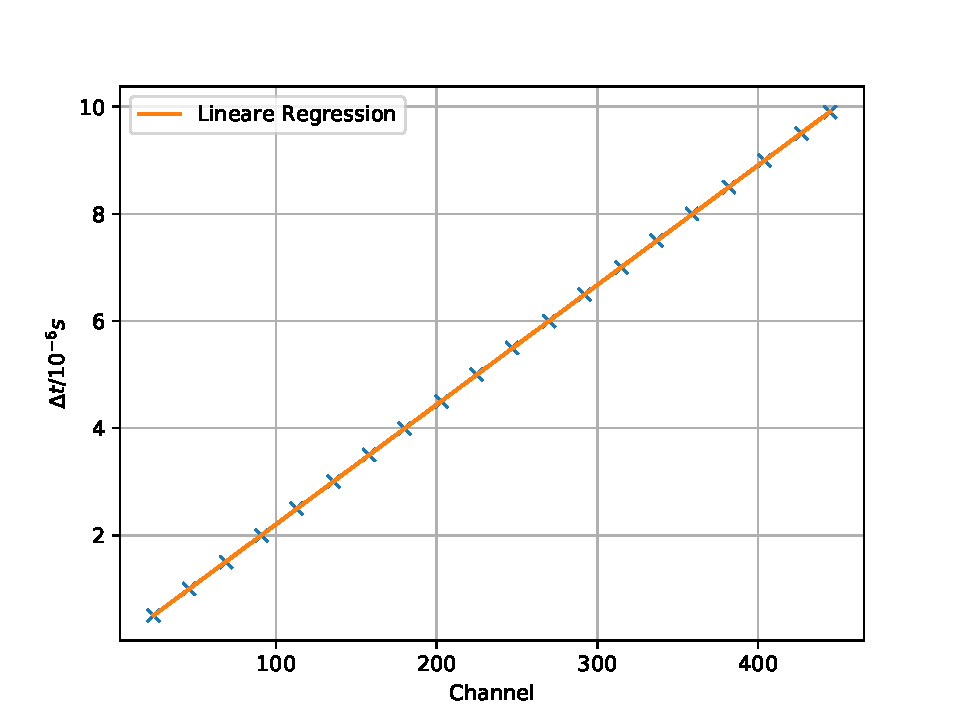
\includegraphics[width=\textwidth]{figkalibrierung.pdf}
  \caption{Kalibrierung des Multi-Channel-Analysers: Zeitlicher Abstand des Doppelimpulses $\Delta$ t gegen den zugehörigen Channel}
  \label{fig:kalibrierung}
\end{figure}
Die lineare Regression hat die Form
\begin{equation*}
  \Delta t = d \cdot C + e
\end{equation*}
und ergibt die folgenden Parameter:
\begin{align*}
  d  &=&  \SI{ 2.2341 \pm 0.0013 e-11}{s}  \\
  e  &=&  \SI{-3.0805 \pm 0.3453 e-11}{s}.  \\
\end{align*}
Mit diesen $d$ und $e$ wird im folgenden aus dem Channel die jeweilige Lebensdauer berechnet.
\FloatBarrier

\subsection{Messung der Lebensdauer}
Die Messdaten zur Lebensdauern der Myonen sind in Abbildung \ref{fig:myonen} aufgetragen.
\begin{figure}[h!]
  \centering
  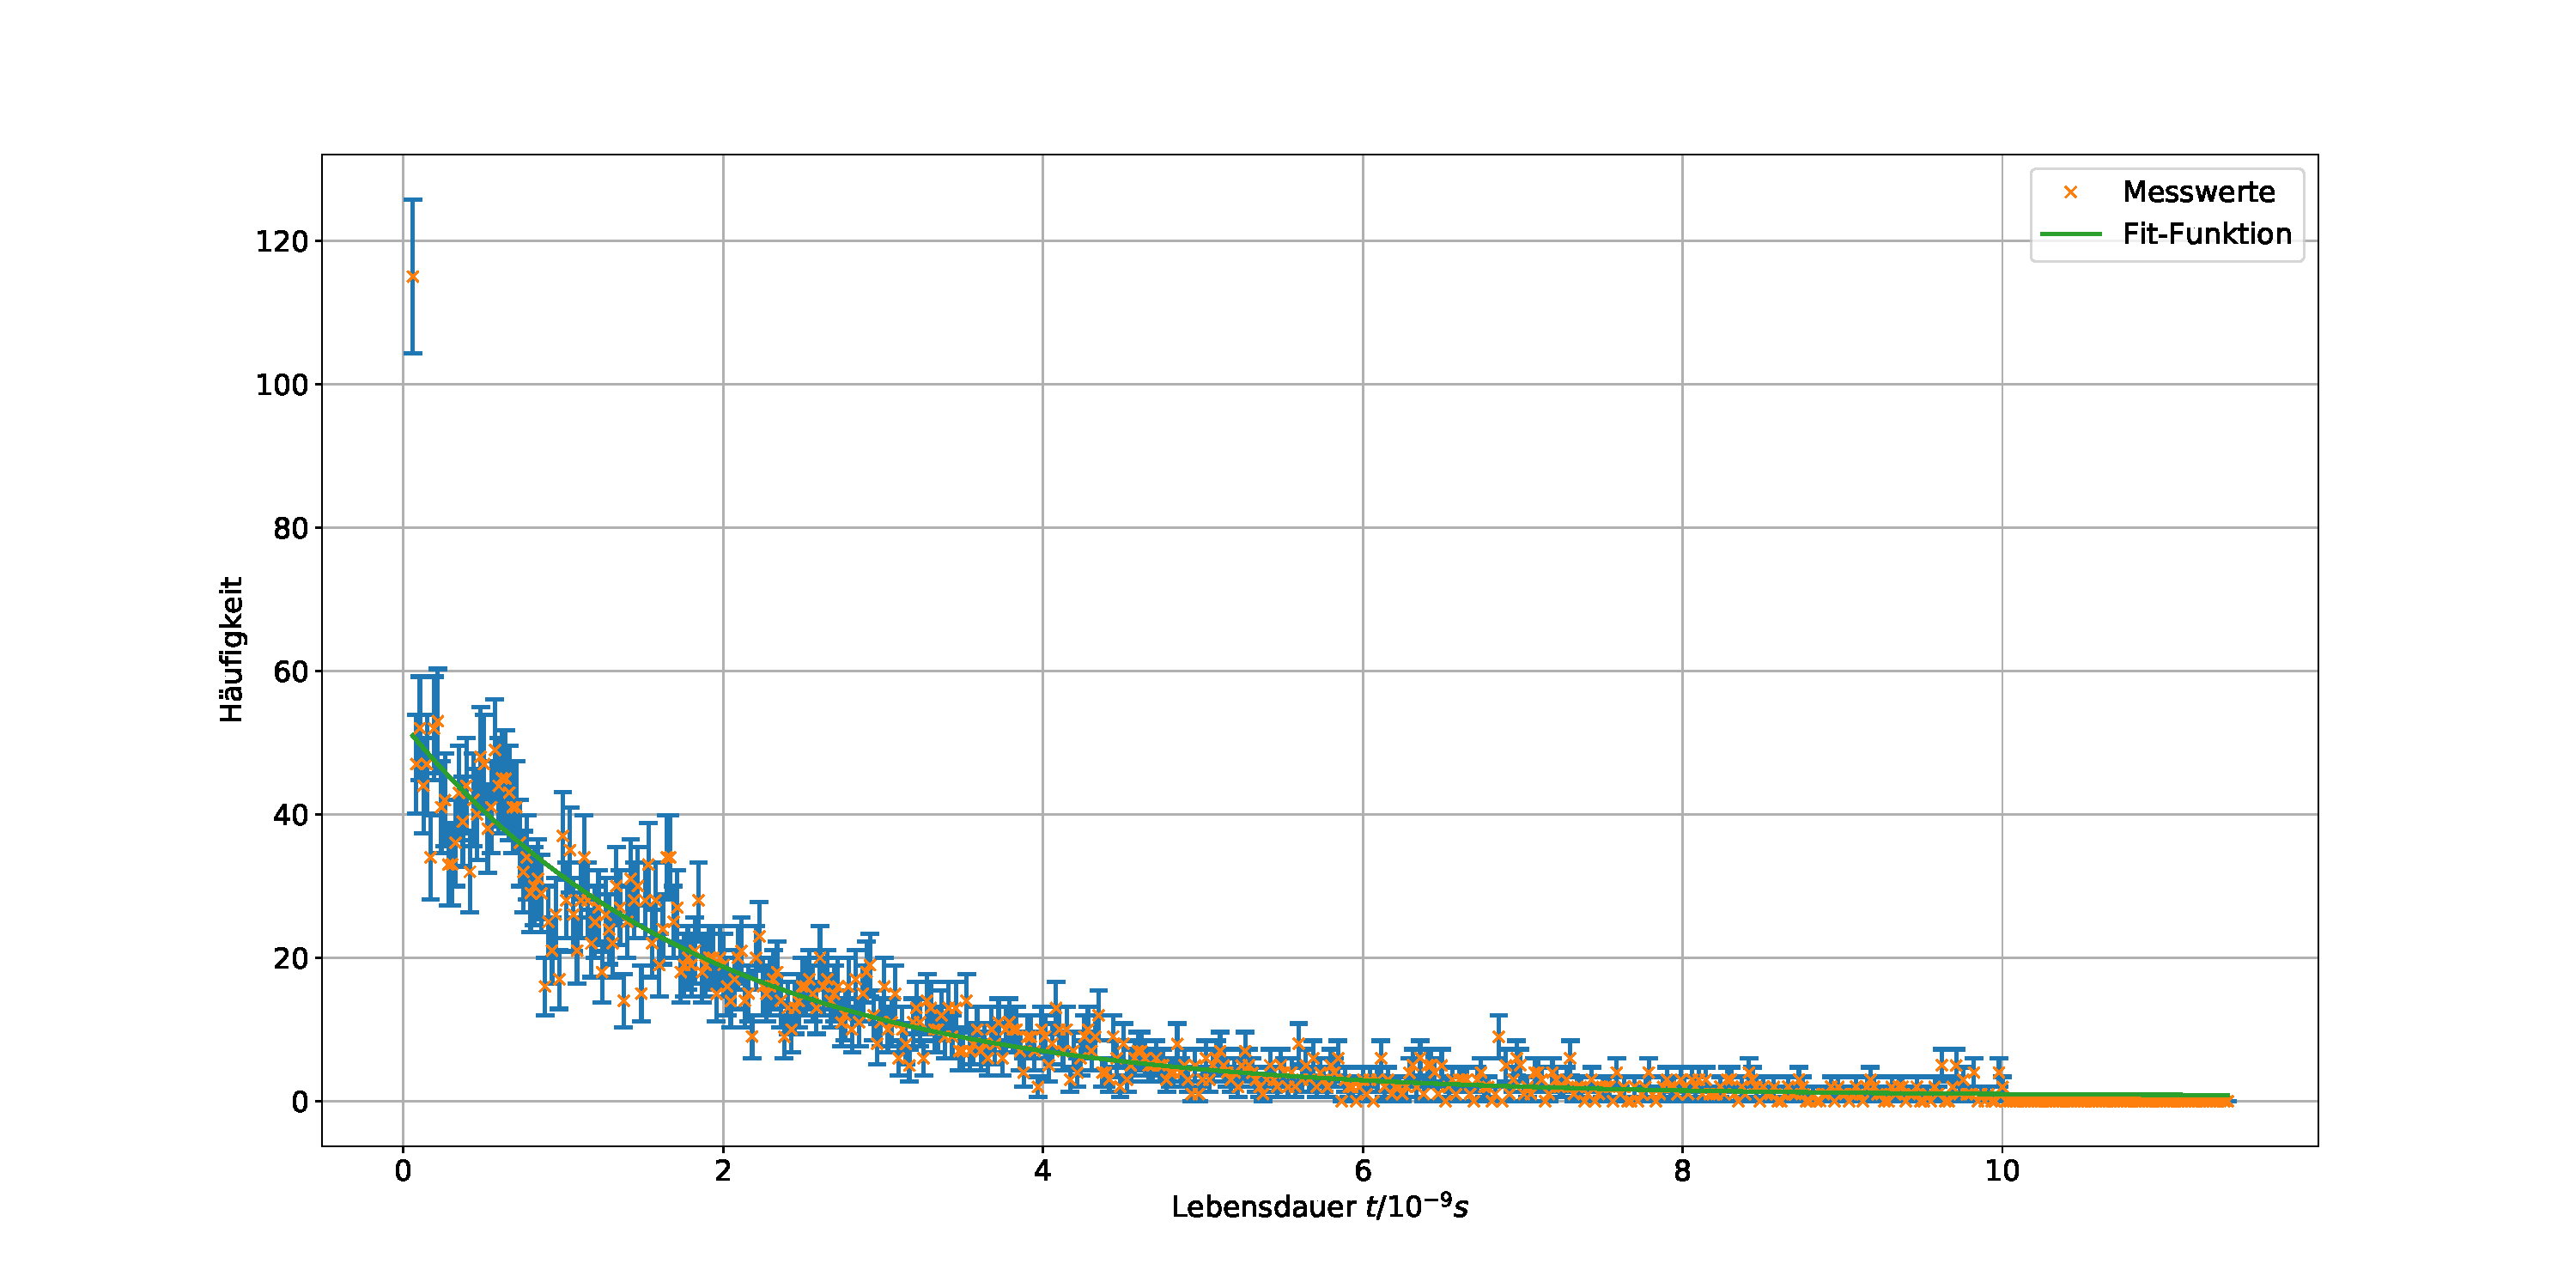
\includegraphics[width=\textwidth]{figmyonen.pdf}
  \caption{Häufigkeit der Myonenzerfälle in Abhängigkeit ihrer Lebensdauer}
  \label{fig:myonen}
\end{figure}
Die Ausgleichsrechnung der Form
\begin{equation*}
  y = f \exp{(-g t)}+h
\end{equation*}
bringt die Parameter
\begin{align*}
  f  &=&  \SI{51.8101 \pm 0.9677}{}\\
  g  &=&  \SI{0.5282 \pm 0.01864 e9}{\frac{1}{s}}\\
  h  &=&  \SI{0.7406 \pm 0.3145}{}.\\
\end{align*}
Aus dem Parameter $g$ wird die Lebensdauer $\tau$ bestimmt:
\begin{equation*}
  \Tau=\frac{1}{g}=\SI{1.8932e-09}{s}
\end{equation*}
\FloatBarrier

%\newpage

\section{Diskussion}
In diesem Experiment geht es darum das magnetische Moment eines Permanentmagneten durch drei verschiedene Methoden zu messen.
\begin{align*}
  \vec{\mu}_{\text{Gravitation}} &=& \SI{0.40753 \pm 0.00109}{A m^2}\\
  \vec{\mu}_{\text{Schwingung}}  &=& \SI{0.4149457 \pm 0.0000001}{A m^2}\\
  \vec{\mu}_{\text{Präzession}}  &=& \SI{0.42515559 \pm 0.000000009}{A m^2}\\
\end{align*}
Die relative Abweichung berechnet sich über
\begin{equation*}
  f_{1,2}=\frac{x_{1}-x_{2}}{x_{2}}.
\end{equation*}
\begin{align*}
  f_{\text{Grav,Schwing}} &=& \SI{1.79}{\%}\\
  f_{\text{Grav,Präz}}    &=& \SI{4.15}{\%}\\
  f_{\text{Schwing,Präz}} &=& \SI{2.40}{\%}\\
\end{align*}
\\Die Abweichung der drei gemessenen Ergebnisse kann verschiedene Gründe haben.
\\Bei der Bestimmung des magnetischen Momentes unter Ausnutzung der Gravitation kommen mehrere Probleme zusammen.
Der Aluminiumstift war bereits vor Beginn des Versuchs verbogen.
Ablesefehler sind nicht auszuschließen.
\\Die Bestimmung des magnetischen Momentes über die Schwingungsdauer des Magneten ist ebenfalls nicht ohne Fehlerquellen.
Messfehler sind auch bei der Schwingungszahl und der Schwingungsdauer möglich.
Die Auslenkung der Billardkugel ist von Messung zu Messung nicht konstant und möglicherweise zu groß.
\\Die Bestimmung des magnetischen Momentes über die Präzession der Billardkugel bringt die meisten Fehlerquellen mit sich.
Es wird beobachtet, dass die Billardkugel sich initial, bereits vor der Auslenkung, mit einer geringen Präzession dreht.
Der Zeitpunkt, an dem die Kugel die richtige Frequenz hat, ist schwierig zu erkennen.
Im Laufe der Messungen wird es auch immer schwieriger, da das Stoboskoplicht sehr anstrengend für die Augen ist.
Es ist nicht auschließbar, dass es bei dem Starten der Uhr und bei dem Aufdrehen der Spulenstromstärke durch Verzögerungen zu fehlerhaften Werten kommt.
Desweiteren gestaltete es sich schwierig, den genauen Zeitpunkt der Umlaufdauer der Präzessionsbewegung zu messen, da die Präzession bei den Messungen zum Teil recht unterschiedliche Auslenkungswinkel hat.



%\begin{figure}
%  \centering
%  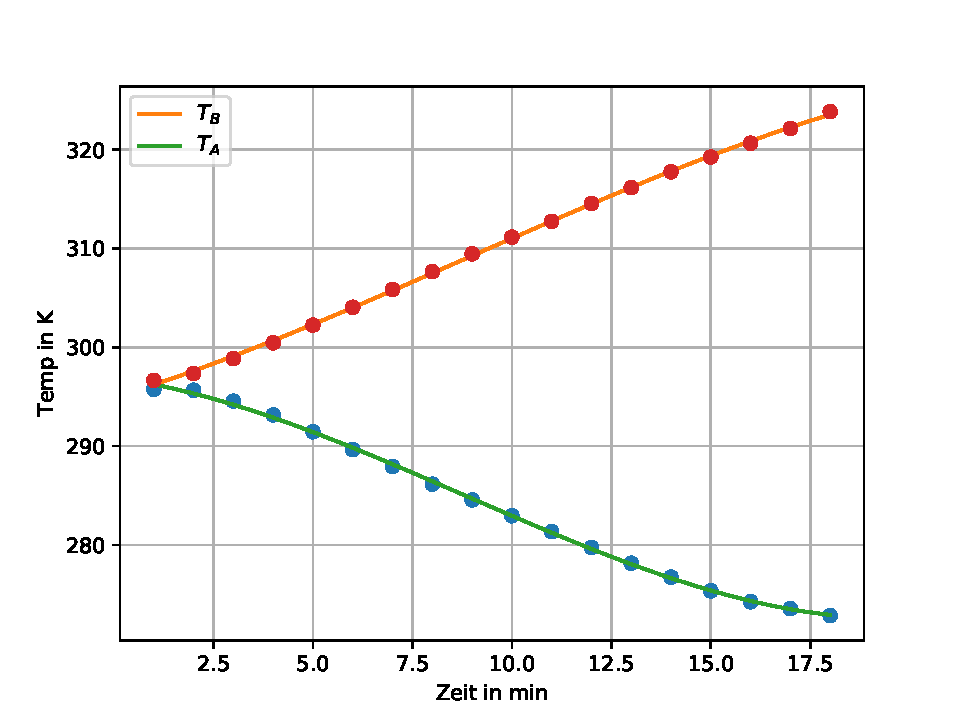
\includegraphics[width=\textwidth]{plot.pdf}
%  \caption{Messung}
%  \label{Messung}
%\end{figure}
%
%\newpage


\nocite{*}
\printbibliography

\begin{figure}
  \centering
  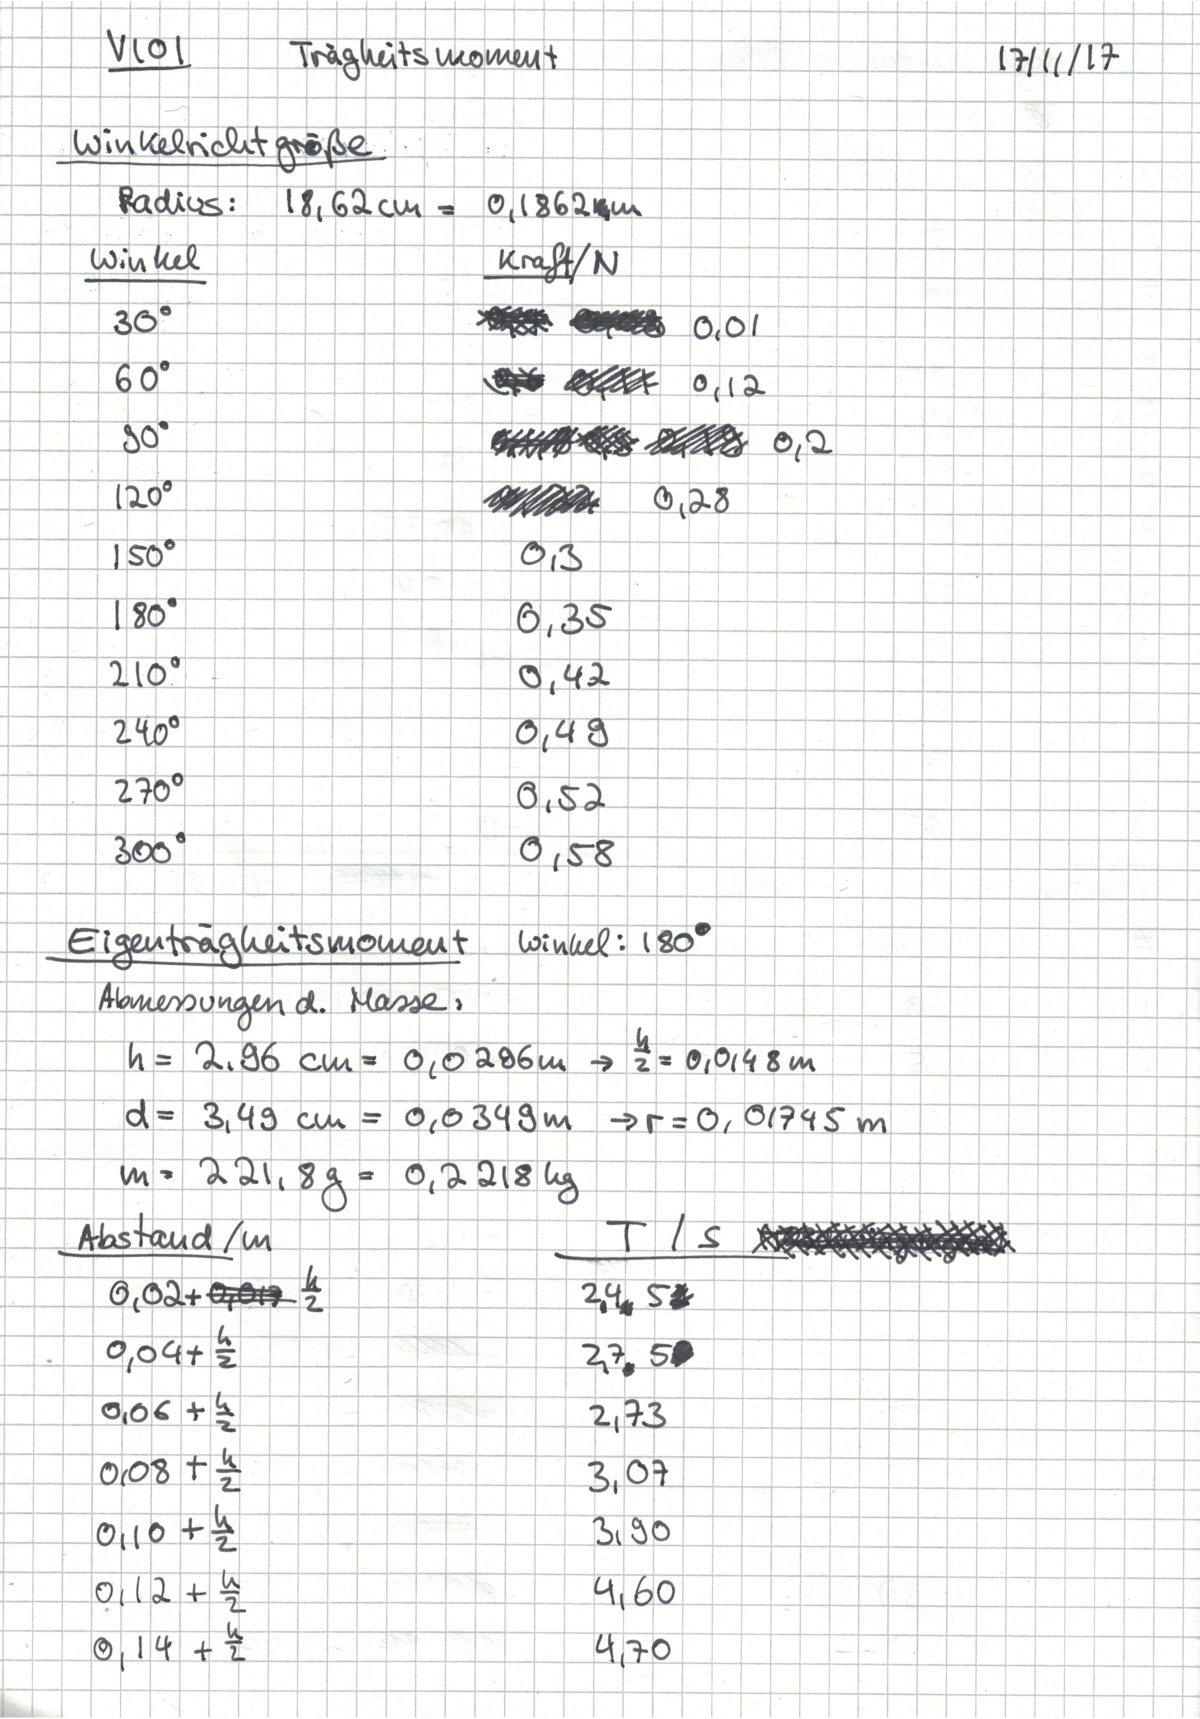
\includegraphics[width=\textwidth]{OMD1.pdf}
  \caption{Originale Messdaten}
  \label{fig:OMD1}
\end{figure}
\begin{figure}
  \centering
  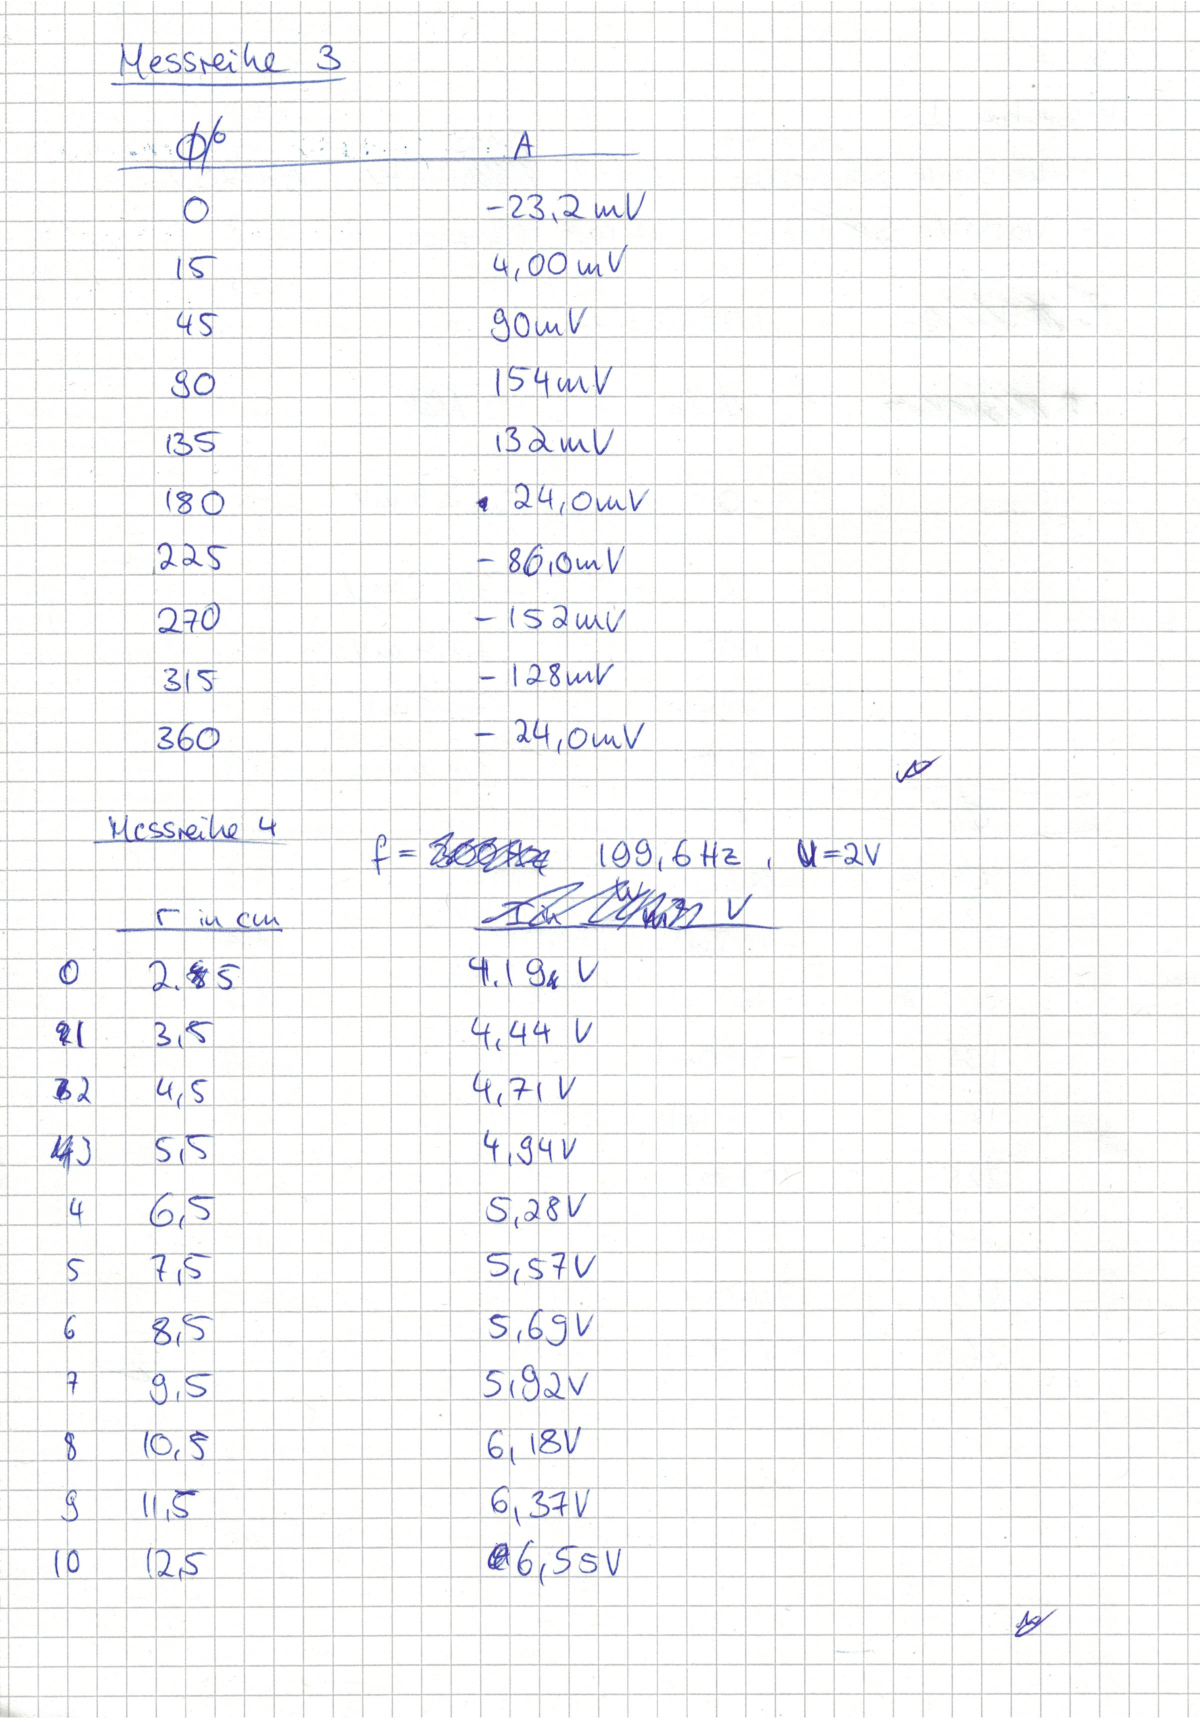
\includegraphics[width=\textwidth]{OMD2.pdf}
  \caption{Originale Messdaten}
  \label{fig:OMD2}
\end{figure}
\begin{figure}
  \centering
  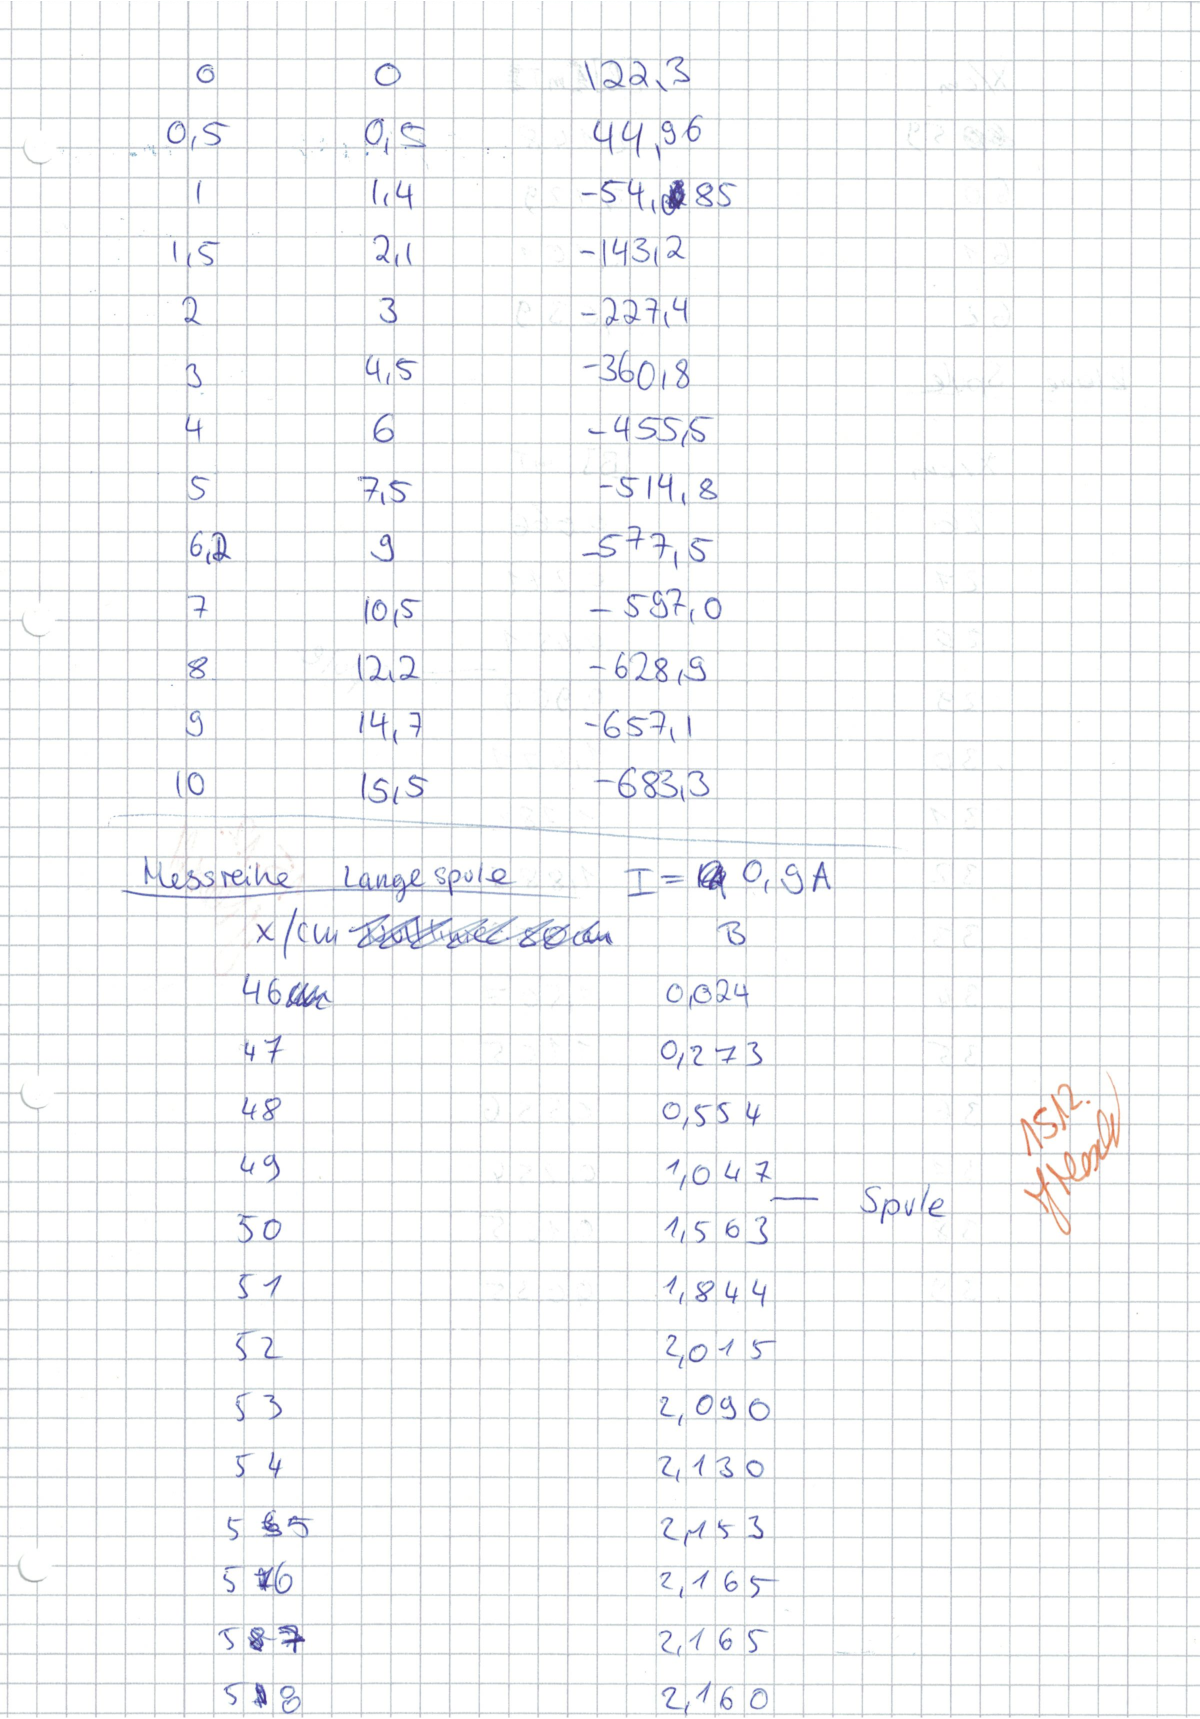
\includegraphics[width=\textwidth]{OMD3.pdf}
  \caption{Originale Messdaten}
  \label{fig:OMD3}
\end{figure}

\end{document}
